% ============================================================
% 第17章：导数的概念——从切线到瞬时变化率
% ============================================================

\chapter{导数的概念——从切线到瞬时变化率}

\begin{applicationbox}
\textbf{学完本章你能做什么？}
\begin{enumerate}
  \item 理解\textbf{导数}是瞬时变化率——切线的斜率
  \item 用定义求简单函数的导数
  \item 掌握基本求导公式
\end{enumerate}
\end{applicationbox}


% ============================================================
\section{从平均变化率到瞬时变化率}
% ============================================================

函数 \(f(x)\) 在区间 \([a, a+h]\) 上的\textbf{平均变化率}：
\[
\frac{f(a+h) - f(a)}{h}
\]

当 \(h \to 0\) 时，平均变化率的极限就是\textbf{瞬时变化率}——导数。

\begin{definitionbox}[导数的定义]
\[
f'(a) = \lim_{h \to 0} \frac{f(a+h) - f(a)}{h}
\]
如果这个极限存在，称 \(f\) 在 \(x=a\) 处\textbf{可导}。

\textbf{用 ε-δ 语言：} 对任意 \(\varepsilon>0\)，存在 \(\delta>0\)，
使得当 \(0<|h|<\delta\) 时，
\[
\left|\frac{f(a+h)-f(a)}{h} - f'(a)\right| < \varepsilon
\]
\end{definitionbox}


% ============================================================
\section{导数的几何意义——切线斜率}
% ============================================================

\begin{examplebox}[1——割线逼近切线]
\begin{center}
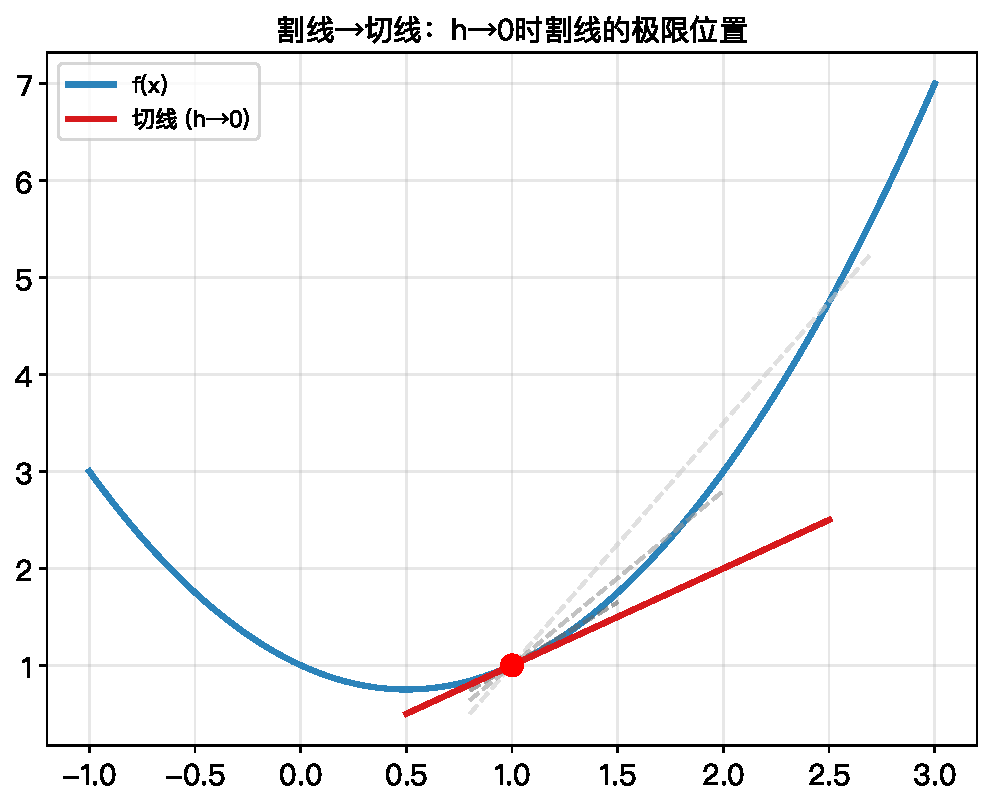
\includegraphics[width=0.7\textwidth]{figures/ch17_tangent.pdf}
\end{center}

割线的斜率：\(\frac{f(a+h)-f(a)}{h}\)\\
当 \(h \to 0\) 时，割线趋近于切线，斜率趋近于导数。
\end{examplebox}

\begin{examplebox}[2——切线斜率 = 导数]
\begin{center}
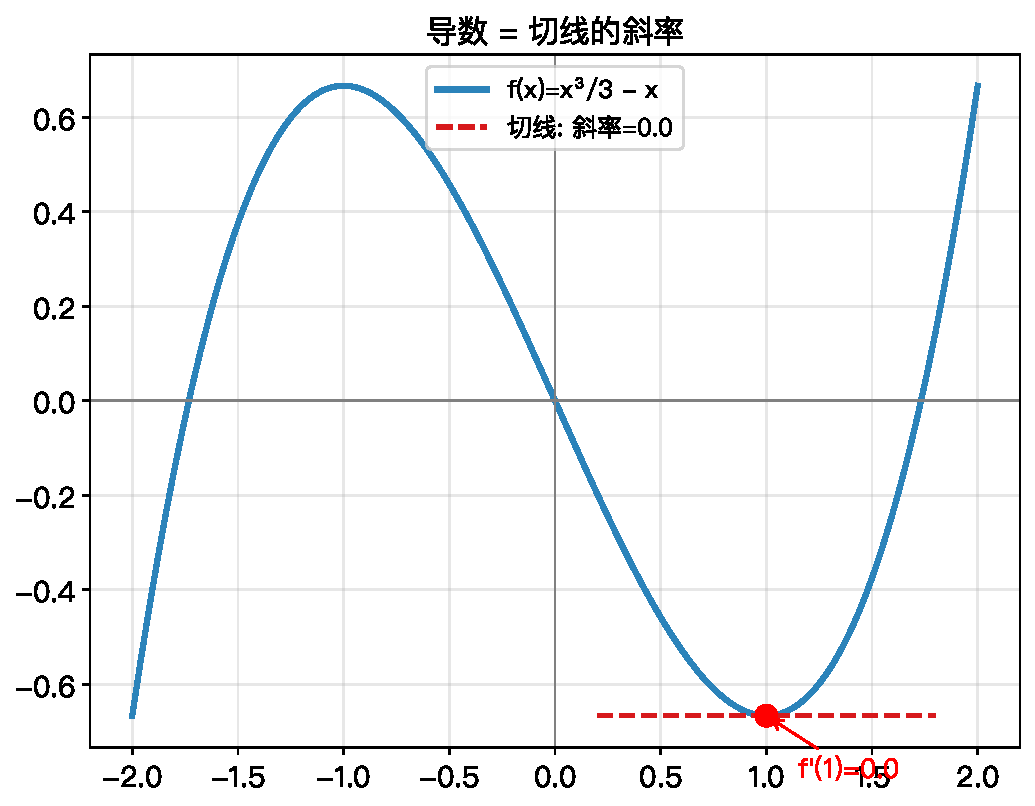
\includegraphics[width=0.7\textwidth]{figures/ch17_derivative_slope.pdf}
\end{center}

\(f(x) = \frac{x^3}{3} - x\)，在 \(x=1\) 处导数 \(f'(1)=0\)——切线水平。
\end{examplebox}


% ============================================================
\section{基本求导公式}
% ============================================================

\begin{theorembox}[基本导数公式]
\begin{align*}
\frac{d}{dx}(c) &= 0 &\text{（常数导数为0）}\\
\frac{d}{dx}(x^n) &= nx^{n-1} &\text{（幂函数）}\\
\frac{d}{dx}(\sin x) &= \cos x \\
\frac{d}{dx}(\cos x) &= -\sin x \\
\frac{d}{dx}(e^x) &= e^x &\text{（最重要的导数！）}\\
\frac{d}{dx}(\ln x) &= \frac{1}{x}
\end{align*}
\end{theorembox}

\begin{examplebox}[3——用定义求导数]
用定义求 \(f(x)=x^2\) 在 \(x=3\) 处的导数：
\[
f'(3) = \lim_{h\to0} \frac{(3+h)^2 - 9}{h}
= \lim_{h\to0} \frac{9 + 6h + h^2 - 9}{h}
= \lim_{h\to0} (6 + h) = 6
\]

由公式：\(f'(x)=2x\)，所以 \(f'(3)=6\)——一致。
\end{examplebox}


% ============================================================
\section{本章小结}
% ============================================================

\begin{progressbox}
\textbf{导数}：\(f'(a) = \lim_{h\to0} \frac{f(a+h)-f(a)}{h}\)

\textbf{几何意义}：切线的斜率

\textbf{基本公式}：\((x^n)'=nx^{n-1}\)，\((\sin x)'=\cos x\)，\((e^x)'=e^x\)，\((\ln x)'=1/x\)

\(e^x\) 的导数等于自己——这是 \(e\) 最重要的性质
\end{progressbox}

% ============================================================
% 习题
% ============================================================
\section{习题}

\begin{exercise}[0]
导数 \(f'(a)\) 的极限定义是什么？
\end{exercise}
\begin{exercise}[0]
导数的几何意义是什么？
\end{exercise}
\begin{exercise}[0]
常数函数的导数是多少？
\end{exercise}
\begin{exercise}[0]
\(e^x\) 的导数是什么？
\end{exercise}

\begin{exercise}[1]
用定义求 \(f(x)=x\) 在 \(x=2\) 处的导数。
\end{exercise}
\begin{exercise}[1]
用定义求 \(f(x)=3\) 的导数。
\end{exercise}
\begin{exercise}[1]
用公式求 \(f(x)=x^5\) 的导数。
\end{exercise}
\begin{exercise}[1]
求 \(f(x)=x^2\) 在 \(x=-1\) 处的导数值。
\end{exercise}

\begin{exercise}[2]
用定义求 \(f(x)=x^3\) 在 \(x=1\) 处的导数。
\end{exercise}
\begin{exercise}[2]
求曲线 \(y=x^2\) 在点 \((2,4)\) 处的切线方程。
\end{exercise}
\begin{exercise}[2]
求 \(f(x)=\sin x\) 在 \(x=0\) 处的导数。
\end{exercise}
\begin{exercise}[2]
求 \(f(x)=\frac{1}{x}\) 在 \(x=2\) 处的导数。
\end{exercise}

\begin{exercise}[3]
用定义求 \(f(x)=\sqrt{x}\) 在 \(x=4\) 处的导数。
\end{exercise}
\begin{exercise}[3]
求曲线 \(y=x^3\) 在 \(x=1\) 处的切线方程。
\end{exercise}
\begin{exercise}[3]
已知 \(f'(2)=5\)，用定义写出极限 \(\lim_{h\to0} \frac{f(2+h)-f(2)}{h}\) 的值。
\end{exercise}
\begin{exercise}[3]
求 \(f(x)=x^4\) 在 \(x=-2\) 处的导数值和切线方程。
\end{exercise}
\begin{exercise}[3]
证明 \((x^2)' = 2x\) 用定义。
\end{exercise}

\begin{exercise}[4]
用定义证明 \((x^n)' = nx^{n-1}\) 对 \(n=3\) 成立。
\end{exercise}
\begin{exercise}[4]
求曲线 \(y=e^x\) 在 \(x=0\) 处的切线方程。
\end{exercise}
\begin{exercise}[4]
求 \(f(x)=\cos x\) 在 \(x=0\) 处的导数。
\end{exercise}
\begin{exercise}[4]
已知 \(f(x)=x^3-2x+1\)，求 \(f'(1)\) 和 \(x=1\) 处的切线方程。
\end{exercise}
\begin{exercise}[4]
证明：若 \(f\) 在 \(x=a\) 处可导，则 \(f\) 在 \(x=a\) 处连续。
\end{exercise}

\begin{exercise}[5]
用定义证明 \((\sin x)' = \cos x\)。
\end{exercise}
\begin{exercise}[5]
求 \(f(x)=\ln x\) 在 \(x=1\) 处的导数。
\end{exercise}
\begin{exercise}[5]
求曲线 \(y=\frac{1}{x}\) 在点 \((1,1)\) 处的切线方程和法线方程。
\end{exercise}
\begin{exercise}[5]
已知 \(\lim_{h\to0} \frac{f(1+h)-f(1)}{h} = 4\)，求 \(f'(1)\)。
\end{exercise}

\begin{exercise}[6]
用定义求 \(f(x)=|x|\) 在 \(x=0\) 处的左右导数，它可导吗？
\end{exercise}
\begin{exercise}[6]
求曲线 \(y=\sqrt{x}\) 上切线斜率为 \(\frac{1}{4}\) 的点。
\end{exercise}
\begin{exercise}[6]
证明：若 \(f\) 是偶函数且可导，则 \(f'\) 是奇函数。
\end{exercise}

\begin{exercise}[7]
用定义求 \(f(x)=\sin x\) 的导数公式，并求出 \(f(x)\) 在 \(x=\frac{\pi}{3}\) 处的切线方程。
\end{exercise}

